\section{Experimental Setups}
\label{sec:experiments}

\begin{figure*}[t]
\centering
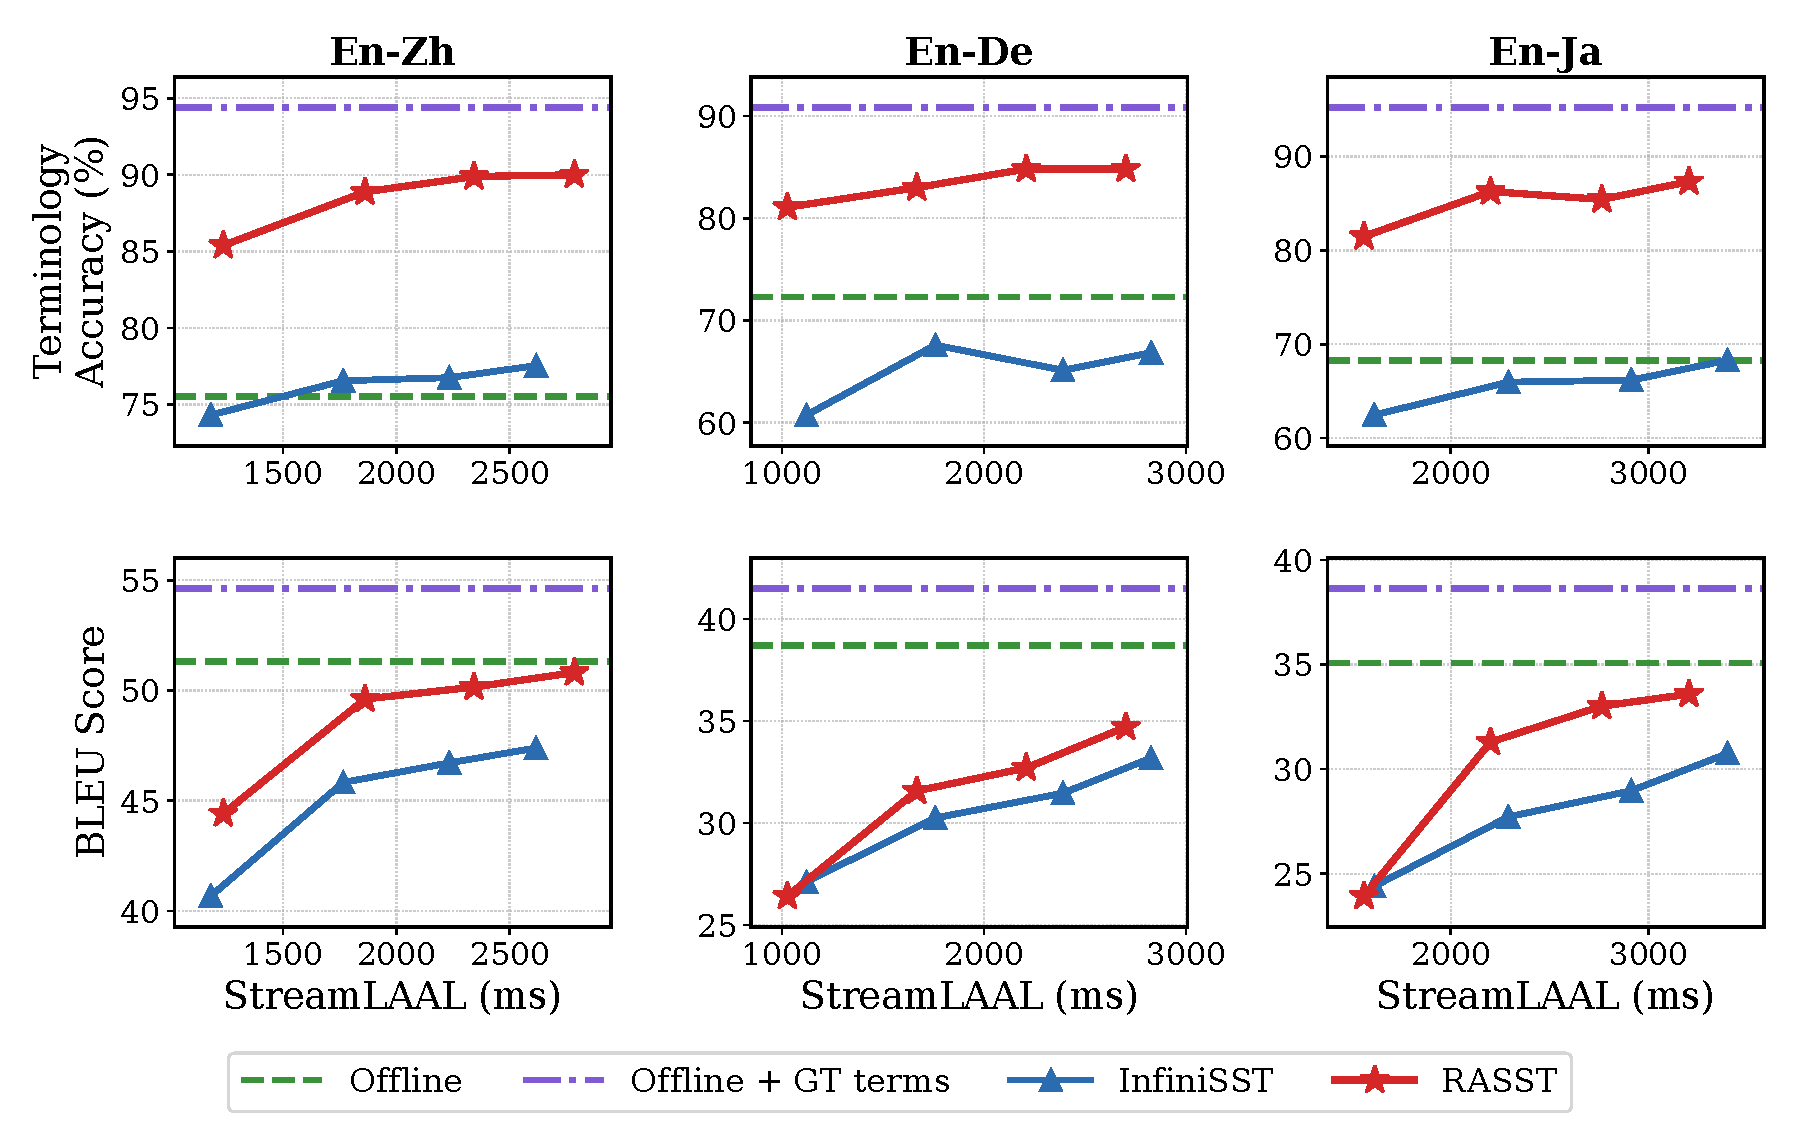
\includegraphics[width=0.9\linewidth]{latex/figures/new_main_result_tagged.pdf}
\caption{Quality–latency trade-off of \method and baselines on the ACL 60/60 dev set. Quality is measured by both terminology accuracy and BLEU. Across all three language directions, \method improves terminology accuracy over InfiniSST by 10\% while also achieving higher translation quality.}
\label{fig:main_result_1}
\end{figure*}

\subsection{Data}
\label{sec:task_datasets}

\paragraph{Retriever Training} We synthesize the retriever training data from GigaSpeech~\citep{chen21o_interspeech} and Wikidata\footnote{\url{https://www.wikidata.org/}}. GigaSpeech is a multi-domain English ASR corpus containing 10K hours of high-quality labeled audio. We process it following the procedure in Section~\ref{sec:retriever}, yielding 4.7M training pairs. The variable speech-context duration is sampled uniformly from ${2.84, 3.96, 4.80, 5.76}$ seconds, corresponding to the inference-time chunk sizes ${0.96, 1.92, 2.84, 3.84}$ plus a $t_\text{lb}=1.92$-second look-back. The look-back captures terms that cross chunk boundaries and we set it to $1.92$ seconds since most terms are shorter than this, as shown in Figure~\ref{fig:term_duration}.

For Wikidata, we extract candidate terms from the Wikidata RDF truthy dump using entities that have both an English \texttt{rdfs:label} and at least one \texttt{wdt:P31} instance-of triple. We normalize each label by removing parenthetical qualifiers, lowercasing for deduplication, and retaining only short alphabetic or hyphenated terms with at most five words. We further require a non-empty short description from the glossary index that does not simply repeat the term, which filters out many ambiguous or non-English labels. To avoid a corpus dominated by very frequent instance types such as people, taxa, or scholarly articles, we assign each entity a primary \texttt{P31} type using its least frequent instance type and rank terms with inverse-type-frequency sampling. Terms appearing in the held-out evaluation glossaries are removed before training. For the resulting top-ranked terms, Gemini-2.5-Flash generates three natural 5--15-word utterance variants that contain the term verbatim using the prompt template in Appendix~\ref{app:wiki_utterance_prompt}; generations that fail this constraint are discarded. We synthesize the utterances with the Fun-CosyVoice3-0.5B-2512 checkpoint of CosyVoice 3, using GigaSpeech speaker prompts.

\paragraph{Speech LLM Training}
We synthesize the Speech LLM training data using the same GigaSpeech ASR dataset. The interleaved En-Zh/De/Ja translation data is synthesized similar to InfiniSST with details in Appendix \ref{sec:speechllm_data_synth}. 
We subsample 12.5K instances for Speech LLM fine-tuning. We build a 100k glossary for distractor retrieval of $G_i$ and we cap the size of $G_i$ at 20. 

\paragraph{Evaluation} We evaluate on two datasets. The first is the ACL 60/60 dev set~\citep{salesky-etal-2023-evaluating}, which contains five English ACL talks translated into 10 target languages. We evaluate on the En-Zh/De/Ja directions, feeding the unsegmented talks directly to the model. This dataset includes human-annotated terminology, which we use to construct the glossary for the model to retrieve from. After deduplication, the glossary contains 238 unique terms. The second is the ESO test set~\citep{eso_dataset}, which consists of five long-form pre-recorded English oncology training videos provided by the European School of Oncology, with translations into French, Spanish, German, and Slovene. We use GPT-5.4\footnote{\url{https://developers.openai.com/api/docs/models/gpt-5.4}} to supplement the dataset with Chinese and Japanese translations, and to extract a candidate terminology list. After manual verification, the resulting glossary contains 217 terms. To test robustness under larger glossaries, we extend both glossaries to 1K and 10K terms with terms drawn from Wikidata that are unseen during training.

\subsection{Evaluation Metrics}
\label{sec:evaluation}

\paragraph{Latency}
Following IWSLT 2025 practice~\citep{agostinelli-etal-2025-findings}, we use StreamLAAL~\citep{papi-etal-2024-streamatt} as our latency metric. StreamLAAL segments the model hypothesis to align with reference sentences and reports the average latency over the resulting (hypothesis, reference) pairs.

\paragraph{Translation Quality}
We evaluate translation quality on the aligned (hypothesis, reference) sentence pairs using SacreBLEU~\citep{papineni-etal-2002-bleu,post-2018-call}.

\paragraph{Terminology Accuracy}
We introduce terminology accuracy to measure how accurately the model translates terms. For each terminology occurrence in the reference, we check whether its translation appears as an exact match in the aligned hypothesis. The metric is the percentage of such occurrences correctly matched, ranging from 0 to 100\%.



\subsection{Model Configuration}
\label{sec:retriever_training}

\paragraph{Architecture}
For the retriever, we use a Qwen3-Omni Audio Transformer\footnote{\url{https://huggingface.co/Atotti/Qwen3-Omni-AudioTransformer}} as the speech encoder, followed by a linear projection. For text encoding, we use the dense BGE-M3\footnote{\url{https://huggingface.co/BAAI/bge-m3}} encoder and extract the feature of \textsc{[CLS]} token. For the Speech LLM, we use Qwen3-Omni-30B-A3B-Instruct\footnote{\url{https://huggingface.co/Qwen/Qwen3-Omni-30B-A3B-Instruct}}.

\paragraph{Training}
We train both the cross-modal retriever and the Speech LLM with LoRA~\citep{hu2022lora}. For retriever training, the number of hard negative $N$ is 1024 and the global batch size is 8192. For Speech LLM training, we use sequence packing and a global batch size of 8192 tokens. Full hyperparameters and details are provided in Appendix~\ref{app:training_details}.
% Dev-only threshold-selection evidence is available at latex/figures/retriever_dev_pr_fixedraw_hn_comparison.pdf.

\paragraph{Inference}

We implement the inference agent in SimulEval~\citep{ma-etal-2020-simuleval}, varying the chunk size $l$ over ${0.96, 1.92, 2.88, 3.84}$ seconds. The Speech LLM is invoked once per chunk and generates up to 40 new tokens per call. We serve it with vLLM~\citep{kwon2023efficient} using tensor parallelism of size 2, decode with temperature $0.6$, top-$p{=}0.95$, and top-$k{=}20$, and strip the assistant's \texttt{<term>} tags from the hypothesis before scoring.

For retrieval, we build a FAISS inner-product index over $\ell_2$-normalized term embeddings. At each step, the retriever encodes the current speech chunk together with a $1.92$-second look-back, and queries the index using only those windows whose right boundary lies within the current chunk. We use Top-$K{=}10$ and discard candidates with similarity below $\tau{=}0.78$\footnote{We select $\tau$ on the dev set to allow at most a 1\% drop in recall.}.


\begin{figure*}[t]
\centering
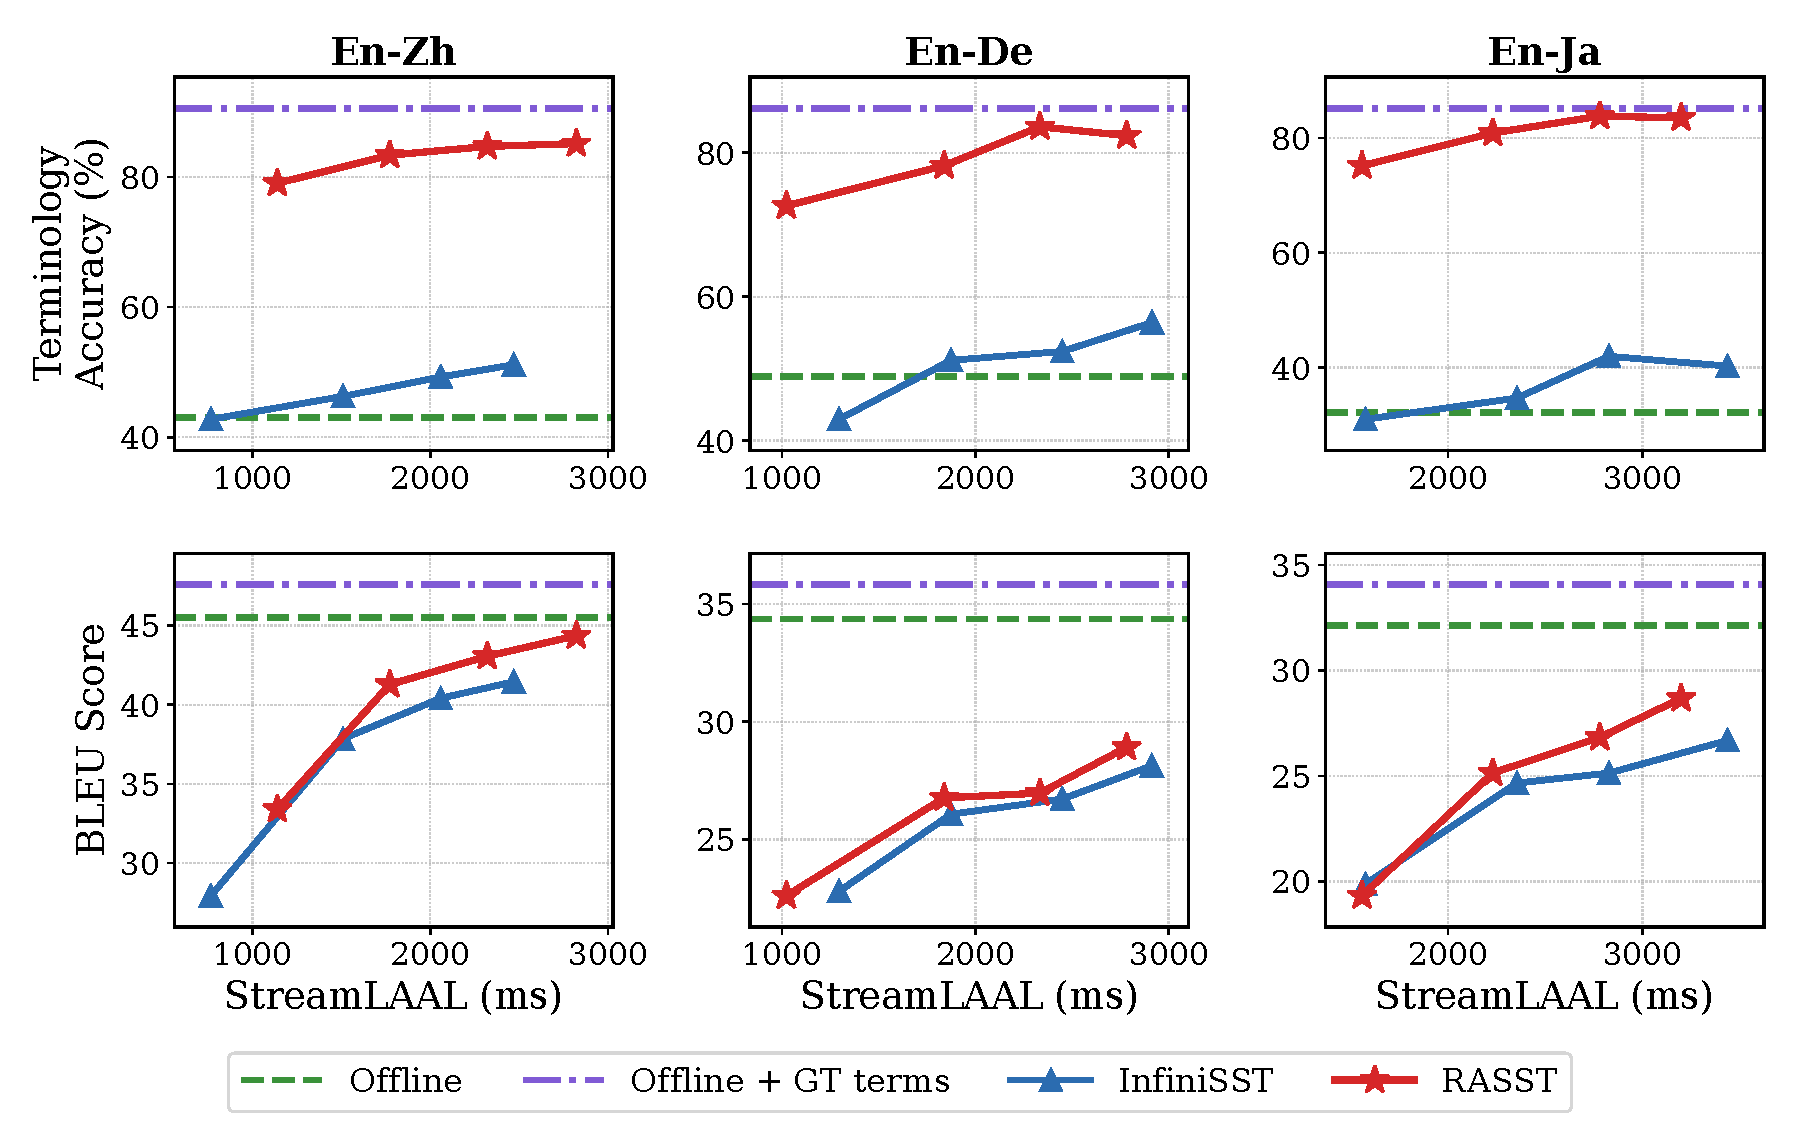
\includegraphics[width=0.9\linewidth]{latex/figures/medicine_main_result.pdf}
\caption{Quality–latency trade-off of \method and baselines on the ESO test set. Quality is measured by both terminology accuracy and BLEU. Across all three language directions, \method improves terminology accuracy over InfiniSST by 30\% while also achieving slightly higher translation quality.}
\label{fig:main_result_2}
\end{figure*}



\begin{figure}[t]
\centering
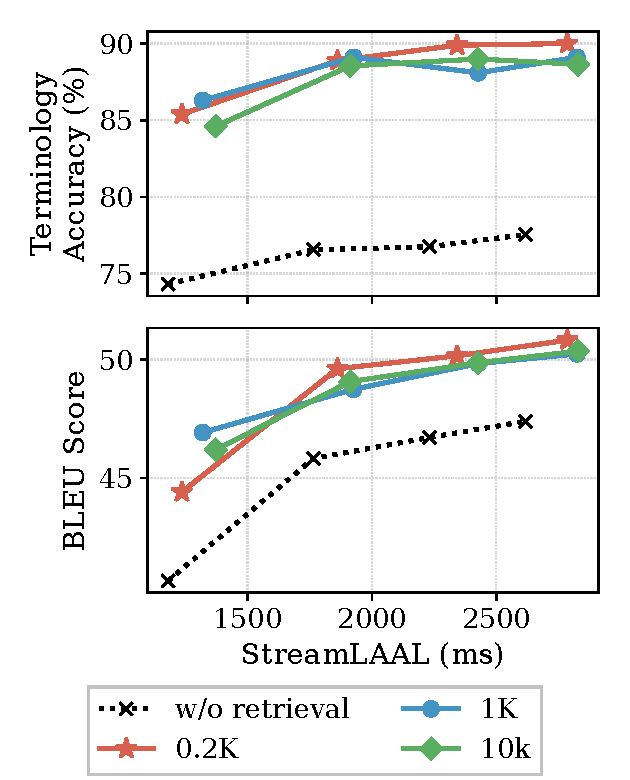
\includegraphics[width=0.8\linewidth]{latex/figures/glossary_bank_ablation_zh_fixedraw.pdf}
\caption{Scaling the glossary from 0.2K to 1K and 10K terms. \method shows only a slight drop in terminology accuracy and translation quality, remaining well above the no-retrieval baseline.}
\label{fig:ablation_glossary_bank}
\vspace{-0.5cm}
\end{figure}


% \begin{figure}[t]
%   \centering
%   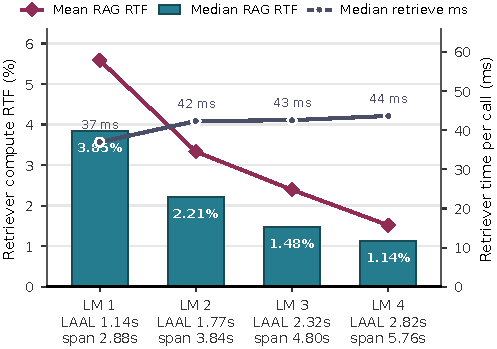
\includegraphics[width=\linewidth]{latex/figures/rag_compute_rtf.pdf}
%   \caption{RTF}
%   %\caption{RAG compute real-time factor under timeline retrieval. We compute $\mathrm{RTF}_{\mathrm{RAG}} = t_{\mathrm{retrieve}} / (0.96\,\mathrm{s}\times\mathrm{LM})$ from verified En-Zh medicine hardraw runtime traces. The retriever runs once per vLLM generation step and encodes the current generation span plus a fixed $1.92\,\mathrm{s}$ look-back. Bars show median per-call RTF, the magenta line shows mean RTF, and the gray line shows median retriever time. Even as the encoded span grows from $2.88$ to $5.76$ seconds, the median RAG compute share falls from $3.85\%$ to $1.14\%$.}
%   \label{fig:rag_compute_rtf}
% \end{figure}

\subsection{Baselines}

\paragraph{Offline}
We use Qwen3-Omni-30B-A3B-Instruct to translate pre-segmented speech utterances offline, with the same decoding parameters as \method. This serves as an upper bound on translation quality.

\paragraph{Offline + GT Terms}
We extend the \textbf{Offline} baseline by adding the ground-truth terms appearing in each utterance to the prompt in a manner similar to \citet{gong24b_interspeech}, helping the model handle terminology correctly. This serves as an upper bound on terminology translation accuracy.

\paragraph{InfiniSST}
InfiniSST~\citep{ouyang-etal-2025-infinisst} is a strong SST baseline for simultaneous translation of unbounded speech and achieved top performance in the low-latency track at IWSLT 2025~\citep{ouyang-etal-2025-cmus,agostinelli-etal-2025-findings}. We train InfiniSST on the same data and with the same Speech LLM as \method, but remove all terminology input $G_i$. This setting can be viewed as \method without retrieval.
